
\section{Marco Te\'orico}

En esta subsecci\'on se introducen conceptos pertinentes al desarrollo del 
trabajo de grado, adem\'as se ha subdividido en tres grandes partes: La primera 
corresponde a los conceptos del Modelado de sistemas; en este caso se hace 
referencia a la estructura y caracter\'isticas que posee Specification and 
Description Language (lenguaje de especificaci\'on y descripci\'on de sistemas), 
conocido por sus siglas en ingl\'es SDL. En la segunda parte se definen algunos 
t\'erminos de las pruebas funcionales de caja negra, y se enfatiza en la 
estructura y caracter\'istica que brinda el lenguaje Testing and Test Control 
Notation version 3 conocido por sus siglas como TTCN-3 para dicha fase; por 
\'ultimo, en la tercera parte se definen algunos conceptos referentes a la 
verificaci\'on formal de sistemas y se hace \'enfasis en la herramienta que se 
va a usar, IFx, definiendo sus caracter\'isticas.

\subsection{Lenguaje para la Especificaci\'on y Descripci\'on de sistemas 
distribuidos}

El uso de un modelo o especificaci\'on formal elimina ambig\"uedades que 
disminuyen los errores dentro del desarrollo del sistema~\cite{Hierons2009}. 
Especificar un sistema por medio de lenguajes formales tiene muchas ventajas 
entre las cuales encontramos: 

\begin{itemize}
 \item Obtener un modelo que tenga una especificaci\'on y descripci\'on clara y 
concisa del sistema.
\item Es posible automatizar la fase de pruebas, con el fin de hacerlas m\'as 
din\'amicas buscando el correcto funcionamiento del sistema.
\item Los sistemas son expresados bajo lenguajes basados en matem\'aticas, lo 
que ayuda a la construcci\'on de sistemas de alta calidad~\cite{Hierons2009}.
\item Es posible usar verificaciones formales para la detecci\'on y 
correcci\'on de errores.
\item Permite ahorrar mucho tiempo/esfuerzo determinando d\'onde se originan 
los errores del sistema.
\end{itemize}

Dentro de los lenguajes que permiten expresar sistemas a partir de su 
especificaci\'on y descripci\'on sin ambig\"uedad, se encuentra SDL, el cual 
posee unas caracter\'isticas atractivas para representar sistemas 
reactivos\footnote{Sistemas reactivos: Son aquellos sistemas que generan una 
salida a partir de  un est\'imulo externo que proviene del ambiente.}, entre 
las cuales se destaca representar sistemas con m\'ultiples agentes a trav\'es 
de m\'aquinas de estados finitas extendidas.

 A continuaci\'on se definir\'an algunas estructuras que posee dicho lenguaje, 
definidas por la recomendaci\'on Z.100 de la ITU-T \cite{SDL2002}: 

\subsubsection{Definiciones en SDL}
\begin{itemize}
 \item Agent (Agente): Es usado para denotar un sistema, bloque o 
proceso que contiene una o m\'as m\'aquinas de estados finitas extendidas.
\item Block (Bloque): Un bloque es un agente que puede contener uno o m\'as 
bloques o procesos paralelos, y podr\'ia tambi\'en contener una o varias 
m\'aquinas de estados finitos extendidas que poseen y manejan datos dentro del 
bloque.
\item Channel (Canal): Un canal es un camino de comunicaci\'on entre dos 
agentes.
\item Environment (Ambiente): El ambiente es el entorno en el que se 
desempe\~na el sistema. 

\item El tipo PID es usado cuando los elementos de datos son referenciados 
a un agente. Existen cuatro variables de tipo PID bien definidas en SDL  las cuales 
son:

\begin{itemize}
 \item SELF: Es el identificador de proceso de la instancia actual.
 \item SENDER: Es el identificador de proceso que envi\'o la \'ultima se\~nal.
 \item PARENT: Es el identificador de proceso que cre\'o la \'ultima instancia.
 \item OFFSPRING: Es el identificador de proceso de la \'ultima instancia 
creada.

\end{itemize}

\item Procedure (Procedimiento): Un procedimiento es una encapsulaci\'on de una 
parte del comportamiento de un agente, que puede ser usado en diferentes partes 
dentro del mismo. Otros agentes puedan hacer llamados a un procedimiento remoto.
\item Signal (Se\~nal): La principal manera de comunicaci\'on es por 
medio de se\~nales que son salidas del agente emisor y entradas al agente 
receptor.
\item State (Estado): Una m\'aquina de estados finita extendida de un 
agente est\'a en un estado si este est\'a esperando por un est\'imulo.
\item Stimulus (Est\'imulo): Un est\'imulo es un evento que puede 
causar que un agente que est\'a en un estado  ejecute una transici\'on.
\item System (Sistema): Un sistema es el agente m\'as exterior que se comunica 
con el ambiente.
\item Timer (Temporizador): Un temporizador es un objeto de propiedad de 
un agente que causa una se\~nal de est\'imulo cuando \'este alcanza un 
determinado tiempo.
\item Transition (Transici\'on): Una transici\'on es una secuencia 
de acciones que un agente realiza hasta que \'este ingresa a un estado.
\item Type/Sort (Tipo): Un tipo es un conjunto de elementos que 
posee caracter\'isticas en com\'un cuya definici\'on puede ser usada para la 
creaci\'on de otras instancias; tambi\'en se pueden formar otros tipos.
\item Value (Valor): El t\'ermino valor es usado para la clase de datos 
que son accesados directamente. Los valores pueden ser pasados con libertad 
entre agentes.

\end{itemize}

\subsubsection{Notaci\'on de SDL}
En SDL existen dos notaciones las cuales son: 

\begin{itemize}
\item SDL/GR   Representaci\'on gr\'afica de SDL (En ingl\'es: Graphic 
Representation form of SDL)
\begin{itemize}
\item Provee elementos gr\'aficos para los conceptos m\'as importantes del 
lenguaje.
\item Tiene una notaci\'on textual para aquellos elementos que no es apropiado 
representarlos gr\'aficamente.
\end{itemize}
\item SDL/PR  Representaci\'on textual de SDL ( En ingl\'es: Textual Phrase 
Representation form of SDL)
\begin{itemize}
\item Usado principalmente para el desarrollo de compiladores.
\end{itemize}
\end{itemize}

La recomendaci\'on de la ITU-T Z.100 enfatiza en la representaci\'on gr\'afica 
de SDL. Adem\'as el software a usar en la fase de modelado del caso de estudio 
brinda la posibilidad de usar SDL/GR. 

La Figura~\ref{fig:SDLGR_PR} es un ejemplo para mostrar la diferencia entre las notaciones SDL/GR y SDL/PR:

\begin{figure}[H]
  \centering
  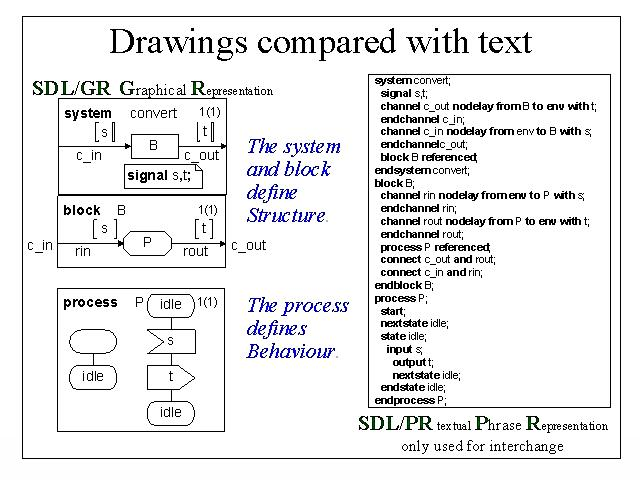
\includegraphics[scale=0.6]{./images/EjemploSDLGR_SDLPR.jpg}
  \caption{Ejemplo comparaci\'on representaci\'on gr\'afica y textual en 
SDL. Fuente \url{http://www.sdl-forum.org/sdl2000present/sld006.htm}}
  \label{fig:SDLGR_PR}
\end{figure}

A partir de este momento los ejemplos relacionados con el modelado de sistemas 
se har\'an por medio de componentes gr\'aficos.

\subsubsection{Requerimientos de especificaci\'on usando Message Sequence Charts 
(MSC)}

En el desarrollo de sistemas Hardware/Software encontramos diferentes etapas en 
las cuales es necesario plantear un requerimiento de especificaci\'on clara y 
concisa, con el fin de elaborar el dise\~no del mismo. Message Sequence Charts 
(MSC)\footnote{Informaci\'on consultada el 20 de Mayo del 2014 en el siguiente 
sitio: \url{http://www.sdl-forum.org/MSC/index.htm.}} es un lenguaje textual y 
gr\'afico que permite expresar requerimientos de especificaciones, simulaci\'on 
y validaci\'on, adem\'as de describir el comportamiento de comunicaci\'on entre las entidades del sistema y el ambiente \cite{Ebner}.  Actualmente existe una relaci\'on directa entre la 
especificaci\'on realizada en un diagrama MSC y SDL, que facilita la parte de 
dise\~no del modelo. 

Las Figuras~\ref{fig:DiagramaMSC} y~\ref{fig:trasl_SDL} muestran un ejemplo de la relaci\'on MSC-SDL.

\begin{figure}[!h]
  \centering
  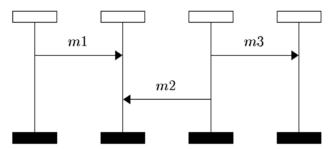
\includegraphics[scale=0.7]{./images/DiagramaMSC.jpg}
  \caption{Diagrama MSC interacci\'on entre cuatro procesos. Fuente~\cite{Reiners} }
  \label{fig:DiagramaMSC}
\end{figure}

\begin{figure}[H]
  \centering
  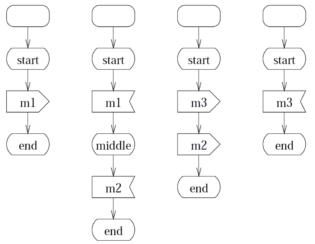
\includegraphics[scale=0.7]{./images/trasl_SDL.jpg}
  \caption{Dise\~no en SDL de la especificaci\'on en MSC. Fuente~\cite{Reiners} }
  \label{fig:trasl_SDL}
\end{figure}

% TESTING


\subsection{Software de Pruebas}
\subsubsection{Terminolog\'ia de pruebas}

Una prueba es un conjunto de actividades que tiene como objetivo identificar 
fallas en un sistema y evaluar su nivel de calidad, para obtener la 
satisfacci\'on del usuario. Esto es un conjunto de tareas con metas claramente 
definidas~\cite{Homes2013}.

De acuerdo al est\'andar ANSI/IEEE 1059 una prueba se puede definir como: Un 
proceso de an\'alisis de un elemento de software para detectar las diferencias 
entre las condiciones existentes y requeridas (es decir defectos / errores / 
fallos) y para evaluar las caracter\'isticas del elemento 
software~\cite{IEEE1994}.

Las pruebas pueden ser est\'aticas o din\'amicas. Las primeras, prueban el 
componente o el sistema a nivel de especificaci\'on o de implementaci\'on sin 
tener que ejecutar \'este~\cite{Ammann2008,Homes2013,ISOIEC29119}. En 
las pruebas din\'amicas, el componente o sistema est\'a en ejecuci\'on y se 
estimula con entradas reales~\cite{Ammann2008,Homes2013}. 

La t\'ecnica de dise\~no de pruebas din\'amicas permite identificar las 
condiciones de la prueba; adicionalmente \'esta se clasifica dentro de tres 
categor\'ias, basadas en c\'omo son derivadas las entradas de las 
pruebas~\cite{ISOIEC29119}. Esas categor\'ias son: Basada en la 
especificaci\'on, 
que consiste en proveer los casos de prueba desde una base de prueba 
describiendo el comportamiento esperado del elemento a 
probar~\cite{ISOIEC29119}; la segunda categor\'ia est\'a basada en la 
estructura, que 
consiste en derivar los casos de prueba desde una caracter\'istica estructural, 
por ejemplo la estructura de un c\'odigo fuente~\cite{ISOIEC29119}. Finalmente 
la tercera categor\'ia corresponde a las pruebas basadas en la experiencia, que 
se basa en un conocimiento previo, bien sea en un sistema en particular o en 
m\'etricas de proyectos previos~\cite{Homes2013}.

Mayoritariamente se emplean dos m\'etodos de pruebas que son: Caja Negra (En 
ingl\'es: Black-Box) y Caja blanca (En ingl\'es: White-Box). El m\'etodo de caja 
negra est\'a basado en los requerimientos y especificaciones para determinar si 
el modelo es correcto o no~\cite{Homes2013,Ammann2008}; una caracter\'istica 
importante de \'este m\'etodo es que no es necesario conocer el sistema interno. 
Por el contrario, el m\'etodo de caja blanca hace parte de la categor\'ia basada 
en la estructura: el caso de prueba se deriva desde el c\'odigo fuente interno 
del modelo~\cite{Ammann2008}; la hip\'otesis fundamental consiste en que el 
modelo cumple con los requerimientos del cliente.  

Los tipos de integraci\'on de pruebas son principalmente dos: De abajo hacia 
arriba (Bottom-up) y de arriba hacia abajo (Top-Down). La primera consiste en 
dise\~nar pruebas que empiecen desde los niveles m\'as finos del sistema a los 
niveles m\'as altos; la integraci\'on Top-Down consiste en dise\~nar pruebas 
desde los niveles m\'as altos del sistema a los m\'as finos.

\subsubsection{TTCN-3 (Testing and Test Control Notation Version 3)}


Para minimizar errores en los sistemas es necesario usar diferentes t\'ecnicas 
que permitan cumplir esta meta; por ejemplo, es \'util realizar las pruebas 
funcionales de caja negra para probar el correcto funcionamiento en las primeras 
etapas del desarrollo del sistema. El presente trabajo de grado pretende usar 
las pruebas funcionales de caja negra en algunos m\'odulos del caso de estudio 
haciendo uso del lenguaje TTCN-3. Parte del modelo arquitect\'onico de TTCN-3 
est\'a soportado por la herramienta RTDS. 

Testing and Test Control Notation Version 3, m\'as conocido por sus siglas en 
ingl\'es como TTCN-3 es un lenguaje de especificaci\'on e implementaci\'on de 
pruebas de tipo caja negra para sistemas distribuidos y 
reactivos~\cite{Grabowski2003}. TTCN-3 se ha construido desde un n\'ucleo de 
lenguaje 
textual que posibilita la interacci\'on con otros lenguajes de descripci\'on, 
por ejemplo SDL~\cite{Grabowski2003,Willcock2011}. Una de las 
caracter\'isticas que presenta TTCN-3 es que su sintaxis textual es similar a 
lenguajes t\'ipicos de programaci\'on, por ejemplo: C, C++ o Java.

\subsubsection{Conceptos b\'asicos de TTCN-3}

\begin{itemize}
\item System Under Test SUT (Sistema Bajo Prueba): Es el sistema el cual se va 
a someter a pruebas.
\item Module (M\'odulo): Es donde est\'a recopilado el c\'odigo TTCN-3 
y se encuentra conformado por: Una parte de definiciones y una parte de 
control~\cite{Willcock2011}.
\item Module definitions part (Parte de definiciones): Especifica las 
definiciones en el nivel superior del m\'odulo; \'estas pueden ser usadas en 
cualquier parte incluso en la parte de control.
\item Module control part (Parte de control): Es la parte principal del 
programa de TTCN-3; en esta parte se describe la secuencia de la ejecuci\'on de 
los casos de prueba (Test cases).
\item Test Cases (Casos de Prueba): Los casos de prueba son especificados en 
la parte de las definiciones del m\'odulo y son llamados en la parte de control. 
Un caso de prueba define el comportamiento que es ejecutado con el fin de 
observar si el sistema pasa la prueba o no~\cite{Grabowski2003}.
\item Test System  (Sistema de Prueba): Ejecuta un caso de prueba y est\'a 
conformado por un conjunto de componentes de prueba interconectados con unos 
puertos de comunicaci\'on bien definidos y una expl\'icita interfaz de sistema 
de prueba (en ingl\'es: Test System Interface, TSI)~\cite{Grabowski2003}.
\item Test Component (Componente de prueba): Ejecuta los casos de prueba (Test 
cases)~\cite{Grabowski2003}.
\item Main Test Component MTC (Componente de prueba principal): La funci\'on 
principal es determinar a trav\'es de los resultados de los componentes de 
prueba si \'esta pasa o no.
\item Verdict (Veredicto): Es una variable impl\'icita que corresponde al 
resultado de la prueba.
\item Matching mechanism (Mecanismo de Coincidencia): TTCN-3 tiene integrado 
un mecanismo de coincidencia que permite evaluar si el sistema satisface ciertas 
condiciones, definidas en los casos de prueba. En TTCN-3 encontramos los 
siguientes valores para el veredicto:
\begin{itemize}
\item Pass: Significa que el SUT se comport\'o de acuerdo al prop\'osito de la 
prueba.
\item Inconc: Significa que no se puede determinar si el SUT pas\'o o fall\'o 
la prueba.
\item Fail: Indica que el SUT no cumpli\'o con el prop\'osito de la prueba.
\item Error: Esta asignaci\'on la hace el ambiente de ejecuci\'on de TTCN-3 
cuando hay fallas en el componente de pruebas o en el SUT.
\item None: Es el valor inicial, cuando el veredicto no ha sido asignado.
\end{itemize}
\item Port (Puerto): Es el lugar donde los mensajes llegan o salen al 
componente de prueba. Un puerto es modelado como una cola infinita tipo FIFO.
\item Template (Plantilla): Son entidades en TTCN-3 usadas para describir el 
contenido de operaciones de comunicaci\'on. Poseen mecanismos de coincidencia 
para los mensajes de llegada y se omite en los mensajes de salida.
\item Alt-statement (Alt-Declaraci\'on): Permite definir distintas operaciones 
de bloqueo, que permiten manejar los mensajes entrantes y determinar si la 
prueba pasa o no.
\item Comunicaci\'on: Se refiere al intercambio de se\~nales entre componentes 
o con el SUT. La comunicaci\'on pueden ser basada en mensajes o basada en 
procedimientos.
\item Comunicaci\'on basada en mensajes: Se intercambian mensajes  con el SUT 
a trav\'es de dos operaciones: send y receive. La operaci\'on send transmite un 
mensaje al SUT a trav\'es de un puerto espec\'ifico. La operaci\'on receive  es 
una operaci\'on de bloqueo que tiene como finalidad comparar el mensaje entrante 
y procede a determinar si coincide con el esperado,para determinar si 
la prueba pasa o no.
\end{itemize}

\subsubsection{Modelo arquitect\'onico del Sistema de Prueba en TTCN-3}

La Figura \ref{fig:modeloTTCN3} representa la arquitectura general del lenguaje 
de TTCN-3. De manera general los adaptadores en TTCN-3 (TTCN-3 Adapters) est\'an 
conformados por un adaptador de sistema y uno de plataforma que sirven para 
implementar funciones externas y adaptar los mensajes al SUT. Por otra parte en 
la capa del ejecutable de TTCN-3 (TTCN-3 Executable) se encuentran componentes 
de manejo (Component Handling), codificaci\'on y decodificaci\'on (Codecs), y 
un ejecutable de TTCN-3. Todo esto sirve para: La distribuci\'on y 
comunicaci\'on entre componentes de prueba en paralelo, la transformaci\'on de 
mensajes a un formato entendible por TTCN-3, y la representaci\'on del 
comportamiento espec\'ifico en el nivel de TTCN-3, respectivamente. Finalmente 
en el Control y Administraci\'on de pruebas (Test Management and Control) se 
encuentran un Administrador de pruebas (Test Management) y una parte para el 
registro de eventos de prueba (Test Logging) que sirven para: proveer control 
sobre el orden de ejecuci\'on de los casos de pruebas, y para el manejo de 
registro de sistema de prueba, respectivamente.

\begin{figure}[!h]
  \centering
  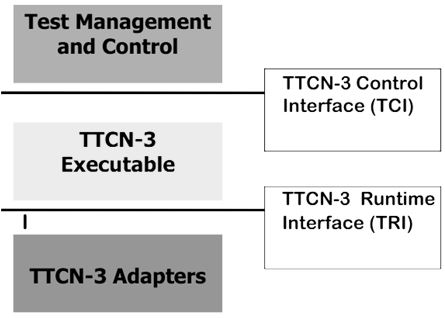
\includegraphics[scale=0.5]{./images/ModeloTTCN3.jpg}
  \caption{Modelo arquitect\'onico simplificado de TTCN-3. Fuente~\cite{Andrus} }
  \label{fig:modeloTTCN3}
\end{figure}

La herramienta RTDS soporta parcialmente la interfaz de control de TTCN-3 (TCI). 
Adicionalmente la interfaz TSI (Test System Interface) es proporcionada por la 
herramienta cuando la prueba se va hacer sobre un sistema descrito en SDL. El 
dise\~no de prueba del caso de estudio se har\'a de forma secuencial para los 
m\'odulos m\'as finos del sistema, con el objetivo de garantizar su correcto 
funcionamiento; por lo tanto, no es de inter\'es en este trabajo de grado 
implementar componentes paralelos de pruebas, lo que implica no hacer uso del 
componente de manejo (Component Handling). Adicionalmente, se aprovechar\'a que 
la herramienta RTDS proporciona impl\'icitamente una interfaz para la 
comunicaci\'on con un SUT descrito en SDL; por lo tanto, tampoco es de inter\'es 
hacer uso de adaptadores para la realizaci\'on de pruebas al sistema.

%M\'etodos formales

\subsection{Verificaciones Formales}

\subsubsection{M\'etodos Formales}

Los m\'etodos formales seg\'un~\cite{Clarke1996} son lenguajes, t\'ecnicas y 
herramientas basados en estructuras matem\'aticas con el objetivo de especificar 
y verificar sistemas. El uso de formalismos en la verificaci\'on de sistemas no 
garantiza que estos est\'en libres de errores, pero brinda la posibilidad de 
expresar modelos sin ambig\"uedades y con un mejor entendimiento.

Dentro de los M\'etodos formales se encuentra la especificaci\'on formal de 
sistemas que consiste en expresar por medio de estructuras de l\'ogica 
matem\'atica las propiedades deseadas, eliminando ambig\"uedades que inducen 
errores en el dise\~no~\cite{Clarke1996}. La especificaci\'on formal es 
una descripci\'on clara y concisa del comportamiento de alto nivel y/o de las 
propiedades del sistema~\cite{Kropf1999}. Por otra parte los m\'etodos 
formales tambi\'en son usados para verificar si el sistema modelado satisface 
ciertas propiedades, que en muchos casos deben de cumplir los sistemas 
cr\'iticos~\cite{Clarke1996}.

\subsubsection{Verificaci\'on Formal de Hardware}

La verificaci\'on de hardware es la demostraci\'on que un circuito o un sistema 
(Nivel de implementaci\'on) se comporta de acuerdo a un conjunto de 
requerimientos (Nivel de especificaci\'on) \cite{Kropf1999}. La 
verificaci\'on formal es contraria a la simulaci\'on, en el sentido que no es 
necesario crear un conjunto de est\'imulos al sistema para garantizar su 
comportamiento. La simulaci\'on es un m\'etodo poco pr\'actico, debido a que no 
es tan sencillo lograr estimular el circuito o el sistema con todas las posibles 
entradas que va a tener durante su funcionamiento. 

Como se muestra en el flujo de dise\~no usando verificaci\'on en la Figura 
\ref{fig:sisVerificacion}, encontramos que para la verificaci\'on de sistemas 
es necesario que el sistema sea especificado de manera rigurosa (System 
specification). Una vez definido el sistema a trav\'es de lenguajes que no 
permitan ambig\"uedades en la descripci\'on,  se definen las propiedades que se 
desea verificar. Paralelo a la definici\'on de las propiedades se puede efectuar 
el proceso de dise\~no (Design Process) hasta obtener un producto o prototipo 
(product or prototype) del sistema deseado. Finalmente, se verifica a trav\'es 
de m\'etodos formales que el prototipo satisface las propiedades definidas 
anteriormente, dando como resultado un \'exito o fallas por medio de 
contraejemplos \cite{Vaovic2005}, como lo hace la t\'ecnica del Model 
Checking.

\begin{figure}[!h]
  \centering
  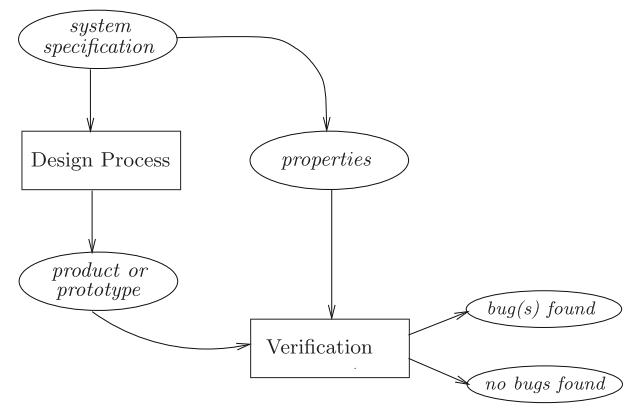
\includegraphics[scale=0.6]{./images/vistaSistemaVerificacion.jpg}
  \caption{Vista general de un sistema de 
verificaci\'on. Fuente:~\cite[p.~3]{Baier2008}}
  \label{fig:sisVerificacion}
\end{figure}

El flujo de dise\~no usando verificaci\'on mostrado anteriormente no est\'a dise\~nado estrictamente para sistemas Hardware, sino que tambi\'en puede ser usado en desarrollo de Hardware/Software.

%Model Checking

\subsubsection{Model Checking}

El Model Checking es una t\'ecnica autom\'atica~\cite{Vaovic2005} de 
verificaci\'on formal que depende de la construcci\'on de un modelo finito del 
sistema y verifica si una propiedad deseada se satisface en dicho 
modelo~\cite{Clarke1996}. La exploraci\'on de todos los posibles estados del 
sistema 
se da de forma exhaustiva.

El Model Checking permite mostrar a trav\'es de contraejemplos los errores del 
modelo, describiendo el camino desde el estado inicial del sistema al estado que 
viola la propiedad que est\'a siendo verificada, lo que facilita la depuraci\'on 
de fallas en el dise\~no del sistema~\cite{Baier2008,Vaovic2005}.

A continuaci\'on se describe el proceso del Model Checking de una forma 
general~\cite{Baier2008}:

\begin{itemize}
 \item Fase del Modelado (Modelling Phase):
 \begin{itemize}
 \item Modelar el sistema por medio de un lenguaje que el Model Checker pueda 
manejar.
 \item Evaluar r\'apidamente el modelo a trav\'es de simulaciones para 
eliminar fallas b\'asicas del modelo.
 \item Especificar la propiedad que se desea verificar en el modelo por medio 
de un lenguaje de especificaci\'on.
 \end{itemize}
 \item Fase de ejecuci\'on (Running phase): En esta fase se ejecuta el model 
checker para verificar si el modelo satisface la propiedad.
\item Fase de an\'alisis (Analysis phase):
\begin{itemize}
\item Si se cumpli\'o la propiedad se contin\'ua verificando las otras en caso 
de haber m\'as.
\item Si la propiedad no se cumpli\'o:
\begin{enumerate}
\item Analizar el modelo con el contraejemplo generado por el model checker.
\item Refinar el modelo, dise\~no o propiedad.
\item Repetir el procedimiento para verificar nuevamente la propiedad.
\end{enumerate}
\item Si se qued\'o corto de memoria: Intentar reducir el modelo e intentar 
nuevamente.
\end{itemize}
\end{itemize}

%IF

\subsubsection{Herramienta IFx}

La herramienta IFx fue desarrollada por investigadores de Verimag en Francia. 
Esta herramienta es un ambiente para el modelado, validaci\'on y verificaci\'on 
de sistemas~\cite{Bozga2004}. 

La herramienta IFx posee caracter\'isticas que proveen grandes ventajas a los 
dise\~nadores de sistemas tales como:

\begin{itemize}
 \item Soporta modelado de alto nivel con formalismos tales como SDL y 
UML.
\item Permite trasladar modelos de alto nivel a una interpretaci\'on 
intermedia conocida como IF.
\item El modelo sem\'antico de IF posee una representaci\'on rica y 
suficientemente expresiva para permitir describir los conceptos b\'asicos y 
estructura del lenguaje fuente.
 \item IF es una representaci\'on intermedia basada en un Aut\'omata 
temporizado extendido, con variables de datos discretas, comunicaci\'on 
primitiva y creaci\'on y destrucci\'on din\'amica de procesos.
\item IF permite la simplificaci\'on de modelos, lo que permite optimizarlo 
para poder ser verificado por medio de la t\'ecnica Model Checking.
\item La propiedad que se desea verificar se puede expresar usando un 
observador (observer) que se puede clasificar como: pure (puro), cut (Poda) o 
intrusive (intrusivo).
\end{itemize}

La Figura \ref{fig:arquiIF} representa la arquitectura IFx\footnote{P\'agina 
oficial de la herramienta IF: \url{http://www-if.imag.fr/index.html}}:

\begin{figure}[H]
  \centering
  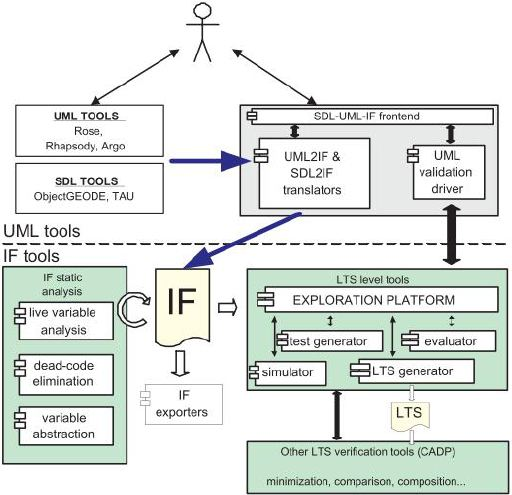
\includegraphics[scale=0.6]{./images/ArquitecturaIF.jpg}
  \caption{Arquitectura de la Herramienta IFx. Tomada de~\cite{Bozga2004}}
  \label{fig:arquiIF}
\end{figure}

El prop\'osito de este trabajo de grado es hacer uso de esta herramienta y no es 
de inter\'es mostrar la interacci\'on de cada componente de dicha herramienta. 
Para saber m\'as respecto de su estructura y sem\'antica referirse 
a~\cite{Bozga2004}.

\subsubsection{Conceptos b\'asicos de IFx}

\begin{itemize}
 \item Process (Proceso): Un proceso describe el comportamiento secuencial 
incluyendo transformaci\'on de datos, comunicaci\'on y creaci\'on de procesos. 
Un proceso se define como un aut\'omata temporizado, que tiene un identificador 
\'unico conocido como pid y una memoria local consistiendo de: variables, 
control de estados y una cola de mensajes que han llegado y no han sido 
consumidos. Para cada instancia de un proceso en SDL la herramienta IFx crea un 
proceso IF.
\item Variables (variables): Cada variable/timer que se declara en SDL es 
traducido al correspondiente proceso IF.
\item States (Estados): Todos los estados del modelo en SDL, incluidos los de 
start y stop, son traducidos dentro de un control de estados estable de IF 
(stable IF Control States). Cada decisi\'on en SDL se traduce en un estado 
inestable (non stable IF state).
\item Transitions (Transiciones): Las transiciones definen el camino entre dos 
estados de control de IF; pueden ser de tres tipos: eager (impaciente) aqu\'i 
las transiciones tienen absoluta prioridad sobre el progreso del tiempo, 
delayable (retardable) pueden permitir el progreso de tiempo mientras est\'a 
habilitada esta transici\'on, lazy (perezoso) no evita el progreso del tiempo.
 \item Observers (Observadores): Los observadores permiten definir la propiedad 
deseada a verificar. En IF podemos definir tres tipos de observadores los cuales 
son~\cite{Bozga2004}:
\begin{itemize}
	\item Pure (Puro): Expresan los requerimientos para ser verificados en el 
sistema.
	\item Cut (Poda): Adicionalmente al observador pure, este permite guiar la 
	simulaci\'on hacia un determinado camino de ejecuci\'on, ayudando a restringir 
	el comportamiento del ambiente.
	\item Intrusive (Intrusivo): Este observador es el m\'as completo de todos, 
	dado que permite manipular el sistema enviando se\~nales y cambiando variables.
\end{itemize}
\end{itemize}

\subsection{Trabajos Relacionados}

La t\'ecnica del Model Checking ha sido usada desde comienzos de los años 90 para la verificaci\'on de propiedades en Hardware. Algunos de los casos m\'as notables en este proceso han sido los siguientes proyectos que se puede encontrar en~\cite{Clarke1996, Woodcock2009}.  En~\cite{Clarke1996} mencionan el proyecto IEEE Futurebus+ como caso de estudio para mostrar las ventajas de la t\'ecnica del Model Checking, usando una herramienta de verificaci\'on autom\'atica por primera vez. Este proyecto consist\'ia en verificar la coherencia de la cache descrita en el est\'andar 896.1-1991 de la IEEE Futurebus+. Este proyecto fue realizado por Clarke y sus estudiantes de la Universidad de Carnegie Mellon. En~\cite{Clarke1996} se pueden encontrar diferentes proyectos tanto en Hardware como en Software donde se usan los m\'etodos formales para garantizar que el sistema cumpla con propiedades cr\'iticas; se puede encontrar adem\'as que el proyecto llamado NewCore fue el primero en ser verificado formalmente en su totalidad, \'este se describ\'ia en 7.500 l\'ineas de c\'odigo en SDL, excluyendo comentarios, que fueron verificados, hallando 112 errores que fueron corregidos.

Compañ\'ias como Intel mencionan que el uso de los m\'etodos formales para la verificaci\'on de hardware ha sido \'util para garantizar sistemas confiables y de alta calidad, adem\'as de permitir mejorar los procesos de desarrollo en sus primeras etapas del sistema~\cite{Fix2008}. 
Recientemente en~\cite{Woodcock2009} se puede encontrar un estado del arte actualizado de las experiencias que han obtenido las industrias en el uso de los m\'etodos formales. La recolecci\'on de informaci\'on se hizo por medio de un cuestionario enviado a las personas que han estado involucradas en el uso de los m\'etodos formales en la construcci\'on de sistemas. La recopilaci\'on de informaci\'on se dio entre Noviembre del 2007 a Diciembre del 2008; a trav\'es de esta encuesta se puede apreciar que la aplicabilidad de los m\'etodos formales no s\'olo es en el campo de la ingenier\'ia, sino tambi\'en, en las finanzas, Salud, Defensa, entre otros.  

Los grupos de investigaci\'on de VERIMAG, que es un centro de investigaci\'on l\'ider en sistemas embebidos, han propuesto un lenguaje intermedio para traducir modelos escritos en SDL y UML para verificar los mismos usando la t\'ecnica de Model Checking. En la literatura encontramos distintos trabajos de grado~\cite{BravoParra2006, Perez2006} que han probado la herramienta de IFx para verificar que algunas propiedades se mantienen en el modelo. En~\cite{BravoParra2006} usaron IFx sobre un sistema de telefon\'ia m\'ovil, como caso de estudio, donde se verificaron algunas propiedades como: la consistencia del tipo de llamada que asigna el sistema con el tipo de llamada que obtiene el usuario. En~\cite{Perez2006} hacen uso de la herramienta IFx para verificar un controlador de sem\'aforos que est\'a descrito en UML, la propiedad que desean probar es: “Se busca s\'i en un momento dado dos sem\'aforos est\'an en verde \'o uno en verde y otro en \'ambar”, lo anterior representa un  estado no deseado del sistema, lo que se concluye es que a trav\'es de la herramienta IFx se pudo determinar la falla del modelo.

En~\cite{Vaovic2005} hacen uso de los m\'etodos formales para verificar propiedades en un caso de estudio referente a redes de comunicaci\'on. El modelado del sistema se hizo por medio de SDL y la verificaci\'on formal fue a trav\'es de la t\'ecnica de Model Checking; se tradujo el modelo de SDL a IF por medio de la herramienta SDL2IF, con el fin de obtener un sistema en un lenguaje al que se le puede aplicar alg\'un model checker. 

En~\cite{Jia2001} plantean y desarrollan un experimento para la verificaci\'on de la capa de control din\'amica del protocolo MASCARA (Mobile Access Scheme based on Contention And Reservation for ATM). Hacen uso de diferentes t\'ecnicas de reducci\'on del sistema, con el objetivo de optimizar el modelo y por ende el tiempo de respuesta usando la t\'ecnica  de Model Checking; para m\'as informaci\'on de las t\'ecnicas usadas ver~\cite{Jia2001}. La forma de diseñar las propiedades a verificar fue de manera incremental, donde se empezaba con propiedades sencillas y se termin\'o verificando la capa de control din\'amica del protocolo MASCARA. Para ver los resultados puede referirse a~\cite{Jia2001}.

En~\cite{MariusMinea} se escogi\'o un bloque del  Software de enrutamiento telef\'onico desarrollado en Alcatel Network Systems Romania, para verificar algunas propiedades. Dicho bloque es el encargado de realizar el tipo de di\'alogo apropiado dependiendo de los par\'ametros de los mensajes de inicio y subsecuentes. El bloque cuenta con dos interfaces: una upstream para el que llama y una downstream para el servidor. En este caso de estudio hacen uso de IF como lenguaje intermedio para aplicar la t\'ecnica de Model Checking y verificar b\'asicamente cuatro propiedades las cuales son: DeadLocks, Progeso, Abortar y Cierre. 

Con respecto a las pruebas funcionales de caja negra usando el lenguaje TTCN-3 encontramos estudios referente al diseño de casos de pruebas a partir de modelos expresados por medio de SDL y MSC. En~\cite{Ebner} proponen una traducci\'on de elementos de MSC a lenguaje de pruebas TTCN-3, en este art\'iculo definen una nueva sem\'antica de MSC para permitir distintas especificaciones de casos de prueba en TTCN-3 que pueden ser concurrentes o no. En~\cite{Willcock2011} hay una breve descripci\'on de c\'omo el lenguaje TTCN-3 ha sido usado para diseñar pruebas al \'ultimo est\'andar de sistemas de comunicaciones m\'oviles conocido como LTE. Se destacan los campos de acci\'on en los cuales el lenguaje TTCN-3 est\'a siendo usado, entre estos encontramos~\cite{Schieferdecker}: sector automovil\'istico,  equipos m\'edicos, distribuci\'on y transmisi\'on de potencia, Finanzas, Aviaci\'on, Ferrocarriles.

Este trabajo de grado pretende hacer uso de una metodolog\'ia que combina dos t\'ecnicas, que son los m\'etodos formales y las pruebas, para la minimizaci\'on de errores en el diseño de sistemas descritos en SDL y pretende verificar algunas propiedades de algunos de sus m\'odulos haciendo uso de la t\'ecnica de Model Checking. Adicionalmente, se desea hacer pruebas funcionales de caja negra por medio del uso del lenguaje TTCN-3 en las primeras etapas del desarrollo del sistema.
 

%ME TO DOLOGIA

\section{Metodolog\'ia de la investigaci\'on}

%El tipo de estudio en el que se enmarca este proyecto es de tipo explicativo y 
%descriptivo. La primera es porque el proyecto de grado trata de aplicar dos 
%t\'ecnicas en una metodolog\'ia que combina, m\'etodos formales y pruebas funcionales de manera %conjunta 
%para minimizar los errores en los sistemas. El aspecto descriptivo est\'a 
%involucrado en mostrar la aplicaci\'on de ambas t\'ecnicas sobre un caso de 
%estudio y haciendo uso de dos herramientas que son: RTDS para el modelado y 
%pruebas e IFx para la verificaci\'on formal.

El proyecto de grado busca aplicar dos t\'ecnicas en una metodolog\'ia que combina, m\'etodos formales y pruebas funcionales de manera conjunta para minimizar errores en el dise\~no de sistemas distribuidos. Para ilustrar la aplicaci\'on de las dos t\'ecnicas se har\'a uso de un caso de estudio empleando dos herramientas que son: RTDS para el modelado y pruebas e IFx para la verificaci\'on formal. Lo anterior implica realizar las siguientes tareas:
%involucrado en mostrar la aplicaci\'on de ambas t\'ecnicas sobre un caso de 
%estudio y haciendo uso de dos herramientas que son: RTDS para el modelado y 
%pruebas e IFx para la verificaci\'on formal.

\begin{enumerate}
\item Comprender el correcto funcionamiento de la herramienta RTDS.
\item Implementar el caso de estudio usando un lenguaje que no introduzca 
errores por ambig\"uedades en la descripci\'on, el cual posteriormente ser\'a 
verificado por medio de m\'etodos formales y pruebas.
\item Determinar en qu\'e etapas del desarrollo de sistemas es pertinente usar 
m\'etodos formales o pruebas.
\item Dise\~nar una bater\'ia de pruebas incrementales que sea apropiada con 
el modelo del caso de estudio y compatible con el lenguaje en el cual ha sido 
expresado.
\item Implementar la bater\'ia de pruebas.
\item Entender el funcionamiento de IFx para verificar formalmente el modelo 
del caso de estudio.
\item Determinar las propiedades cr\'iticas del sistema que se desea verificar.
\item Seleccionar los tipos de observadores para la especificaci\'on de la 
propiedad a verificar.
\item Seleccionar las propiedades a verificar.
\item Implementar los observadores.
\end{enumerate}


\section{Resultados esperados}

Se espera mostrar a trav\'es de un caso de estudio, que es posible minimizar los 
errores en el dise\~no de \'este usando la combinaci\'on de los m\'etodos 
formales y Pruebas sobre distintas etapas del dise\~no del caso de estudio.

\section{Descripci\'on de recursos}

\subsection{Director}

\begin{itemize}
 \item Eugenio Tamura Morimitsu.\\
 Dr. en Arquitectura y Tecnolog\'ia de los Sistemas Inform\'aticos.
 
\end{itemize}

\subsection{Recursos T\'ecnicos}

\begin{itemize}
 \item Computador personal
 \item Material bibliogr\'afico (Revistas, libros)
 \item Papeler\'ia (Impresiones)
\item Conexi\'on a internet
\item Herramienta Real Time Developer Studio 
\item Herramienta IFx
\end{itemize}

\subsection{Presupuesto}

Para llevar a cabo el trabajo de grado planteado se ha realizado la siguiente 
tabla detallando el valor de dicho proyecto, considerando que la duraci\'on para 
su realizaci\'on es de 28  semanas:

\begin{table}[H]
  \centering
  \begin{tabular}{|l|c|r|}
    \hline \hline
    \textbf{Detalle} & \textbf{Costo por tiempo} & \textbf{Costo} \\ 
    \hline
    Investigador                   & 480.000/semana & 13'440.000 \\ \hline
    Computador Personal            & 25.000/semana & 700.000\\ \hline
    Material Bibliogr\'afico       & 500.000/Investigaci\'on & 500.000\\ \hline
    Papeler\'ia  & 120.000/Investigaci\'on & 120.000\\ \hline
    Conexi\'on a Internet & 15.000/semana& 420.000 \\ \hline
    \hline
    \hfill &  \textbf{Total}           & 15'180.000 \\
    \hline
  \end{tabular}
  \caption{Presupuesto}
  \label{tab:presupuesto}
\end{table}

\section{Tabla de Contenido}

\begin{enumerate}
	\item Introducci\'on
	\begin{enumerate}[{1}.1.]
		\item Motivaci\'on
		\item Objetivos, alcances y limitaciones
		\item Metodolog\'ia de estudio
		\item Contribuciones  
		\item Estructura del Documento
	\end{enumerate}
	\item Marco de Referencia
	\begin{enumerate}[{2}.1.]
		\item Estado del Arte
		\item El lenguaje SDL
		\begin{enumerate}[{2}.2.1.]
		      \item Conceptos b\'asicos de SDL 
		      \item Ejemplo
		\end{enumerate}
		\item El Lenguaje TTCN3
		\begin{enumerate}[{2}.3.1.]
		      \item Conceptos b\'asicos de TTCN3 
		      \item Ejemplo
		\end{enumerate}
		\item La herramienta RTDS
		\item La herramienta IFx
		\begin{enumerate}[{2}.5.1.]
		      \item Conceptos b\'asicos del lenguaje IFx  
		      \item Ejemplo
		\end{enumerate}
	\end{enumerate}
	\item Caso de estudio del proyecto de grado
	\begin{enumerate}[{3}.1.]
		\item Modelado 
		\item Pruebas 
		\item Verificaci\'on formal a m\'odulos 
	\end{enumerate}
	\item Resultados obtenidos
	\begin{enumerate}[{4}.1.]
		\item An\'alisis y Discusi\'on
	\end{enumerate}
	\item Observaciones Finales
	\begin{enumerate}[{5}.1.]
		\item Conclusiones
		\item Trabajos futuros
	\end{enumerate}
	\item Bibliograf\'ia
	\item Anexos
\end{enumerate}

\section{Cronograma}

\noindent En la Figura \ref{fig:cronograma} se observa el cronograma de
actividades por semanas. La reuni\'on con el director del proyecto de grado se
realizar\'a cada 15 d\'ias.


\begin{landscape}
    \begin{figure}[!h]
        \centering   
            \vspace*{2 cm}
            \scalebox{0.8}{
                 
\begin{gantt}[xunitlength=0.5cm,fontsize=\small,titlefontsize=\small,
drawledgerline=true]{21}{28}

    \begin{ganttitle}
      \titleelement{Semanas}{28}
    \end{ganttitle}
    
    \begin{ganttitle}
      \numtitle{1}{1}{28}{1}
    \end{ganttitle}
   
    \ganttbar{Asesor\'ia con el director del trabajo de grado}{0}{28}
   
    \ganttbar{Revisi\'on bibliogr\'afica}{0}{13}
     
    \ganttgroup{Investigaci\'on para desarrollo proyecto de grado}{0}{19}
    \ganttbar{Investigaci\'on acerca de Modelado de Sistemas (Usando \textbf{SDL y MSC})}{0}{5}
    \ganttbarcon{Investigaci\'on acerca de Pruebas a Modelos en SDL}{5}{6}
    \ganttbarcon{Investigaci\'on M\'etodos Formales para Verificaci\'on}{12}{7}
   
   % Elaboracion anteproyecto 
    \ganttgroup{Elaboraci\'on propuesta de trabajo de Grado}{19}{7}
    \ganttbar{Elaboraci\'on de Ante Proyecto}{19}{3}
    \ganttbarcon{Entrega de Ante proyecto Facultad de Ingenier\'ia}{23}{1}
    \ganttbarcon{Aprobaci\'on Ante Proyecto}{24}{3}
    
    \ganttgroup{Desarrollo Caso de Estudio}{6}{21}
    \ganttbar{Modelado del caso de estudio usando SDL en RTDS}{6}{6}
    \ganttbarcon{Documentaci\'on del Modelado del caso de estudio}{12}{1}
    \ganttbarcon{Elaboraci\'on de pruebas usando TTCN-3 al caso de estudio}{15}{6}
    \ganttbarcon{Documentaci\'on de las pruebas elaboradas al caso de estudio}{21}{1}
    \ganttbarcon{Verificar distintos m\'odulos del caso de estudio}{22}{3} 
    \ganttbarcon{Documentaci\'on de la verificaci\'on del caso de estudio}{25}{1} 
    
	% documentacion proyecto    
    
   
    \ganttbar{Organizar,Redactar y Entregar la monograf\'ia a la Facultad de Ingenier\'ia}{26}{2}
   
    
    %\ganttcon{20}{5}{20}{8}
    
  \end{gantt}


            }
        \caption{Cronograma}
        \label{fig:cronograma}
    \end{figure}
\end{landscape}
